% fan_in.tex
% ══════════════════════════════════════════════════════
% Fan-in / many-to-one network diagram
% Matches the uploaded image:
%   - 5 coloured input nodes on the left
%   - Lines converge to a mid junction point
%   - Single output node (yellow) on the right
% ══════════════════════════════════════════════════════

\documentclass[tikz, border=10pt]{standalone}
\usepackage{tikz}
\usetikzlibrary{calc}

% ── Palette (matching the image) ─────────────────────
\definecolor{bg teal}    {HTML}{8BBFC4}   % background
\definecolor{navy}       {HTML}{1D4E6B}   % line / border color
\definecolor{col salmon} {HTML}{C97B5E}   % input node 1
\definecolor{col green}  {HTML}{6AAF5E}   % input nodes 2,3,4
\definecolor{col teal}   {HTML}{5A9E8F}   % input node 5
\definecolor{col yellow} {HTML}{E8C84A}   % output node

\begin{document}
	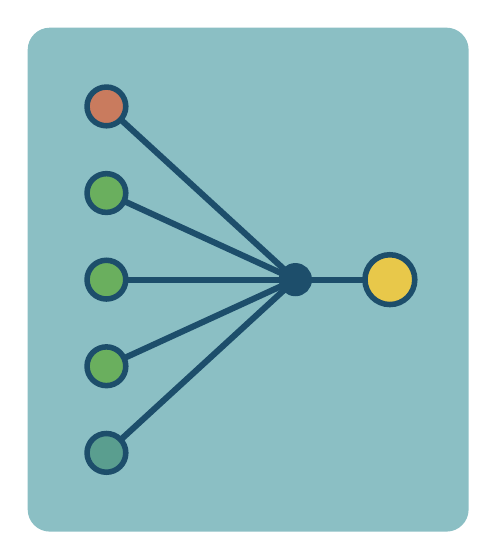
\begin{tikzpicture}[
		% ── shared node style ──────────────────────────────
		net node/.style={
			circle,
			draw        = navy,
			line width  = 2pt,
			minimum size= 14pt,
			inner sep   = 0pt,
		},
		% ── line style ─────────────────────────────────────
		net edge/.style={
			draw        = navy,
			line width  = 2.2pt,
			line cap    = round,
		},
		]
		
		% ── Background ─────────────────────────────────────────
		\fill[bg teal, rounded corners=8pt]
		(-1.0,-3.2) rectangle (4.6, 3.2);
		
		% ── Coordinates ────────────────────────────────────────
		% Input nodes: x=0, evenly spaced vertically
		\coordinate (i1) at (0,  2.2);   % salmon
		\coordinate (i2) at (0,  1.1);   % green
		\coordinate (i3) at (0,  0.0);   % green
		\coordinate (i4) at (0, -1.1);   % green
		\coordinate (i5) at (0, -2.2);   % teal
		
		% Junction / convergence point (where all lines meet)
		\coordinate (junc) at (2.4, 0.0);
		
		% Output node
		\coordinate (out) at (3.6, 0.0);
		
		% ── Edges (draw before nodes so nodes sit on top) ──────
		\foreach \i in {i1,i2,i3,i4,i5}{
			\draw[net edge] (\i) -- (junc);
		}
		% Short segment from junction to output
		\draw[net edge] (junc) -- (out);
		
		% ── Input nodes ────────────────────────────────────────
		\node[net node, fill=col salmon] at (i1) {};
		\node[net node, fill=col green]  at (i2) {};
		\node[net node, fill=col green]  at (i3) {};
		\node[net node, fill=col green]  at (i4) {};
		\node[net node, fill=col teal]   at (i5) {};
		
		% ── Junction dot (navy filled, slightly larger) ─────────
		\node[net node, fill=navy, minimum size=10pt] at (junc) {};
		
		% ── Output node ────────────────────────────────────────
		\node[net node, fill=col yellow, minimum size=18pt] at (out) {};
		
	\end{tikzpicture}
\end{document}